\documentclass{article}

\usepackage{fancyhdr}
\usepackage{extramarks}
\usepackage{amsmath}
\usepackage{amsthm}
\usepackage{amsfonts}
\usepackage{tikz}
\usepackage[plain]{algorithm}
\usepackage{algpseudocode}
\usepackage{listings}
\usepackage{xcolor}
\usepackage[english]{babel}
\usepackage[T1]{fontenc}
\usepackage{lmodern,mathrsfs}
\usepackage{xparse}
\usepackage[inline,shortlabels]{enumitem}
\setlist{topsep=2pt,itemsep=2pt,parsep=0pt,partopsep=0pt}
\usepackage[dvipsnames]{xcolor}
\usepackage[utf8]{inputenc}
\usepackage[a4paper,top=0.5in,bottom=0.2in,left=0.5in,right=0.5in,footskip=0.3in,includefoot]{geometry}
\usepackage[most]{tcolorbox}
\tcbuselibrary{minted} % tcolorbox minted library, required to use the "minted" tcb listing engine (this library is not loaded by the option [most])
\usepackage{minted} % Allows input of raw code, such as Python code
% \usepackage[colorlinks]{hyperref}



\usetikzlibrary{automata,positioning}

%
% Basic Document Settings
%

\tcbset{
    pythoncodebox/.style={
        enhanced jigsaw,breakable,
        colback=gray!10,colframe=gray!20!black,
        boxrule=1pt,top=2pt,bottom=2pt,left=2pt,right=2pt,
        sharp corners,before skip=10pt,after skip=10pt,
        attach boxed title to top left,
        boxed title style={empty,
            top=0pt,bottom=0pt,left=2pt,right=2pt,
            interior code={\fill[fill=tcbcolframe] (frame.south west)
                --([yshift=-4pt]frame.north west)
                to[out=90,in=180] ([xshift=4pt]frame.north west)
                --([xshift=-8pt]frame.north east)
                to[out=0,in=180] ([xshift=16pt]frame.south east)
                --cycle;
            }
        },
        title={#1}, % Argument of pythoncodebox specifies the title
        fonttitle=\sffamily\bfseries
    },
    pythoncodebox/.default={}, % Default is No title
    %%% Starred version has no frame %%%
    pythoncodebox*/.style={
        enhanced jigsaw,breakable,
        colback=gray!10,coltitle=gray!20!black,colbacktitle=tcbcolback,
        frame hidden,
        top=2pt,bottom=2pt,left=2pt,right=2pt,
        sharp corners,before skip=10pt,after skip=10pt,
        attach boxed title to top text left={yshift=-1mm},
        boxed title style={empty,
            top=0pt,bottom=0pt,left=2pt,right=2pt,
            interior code={\fill[fill=tcbcolback] (interior.south west)
                --([yshift=-4pt]interior.north west)
                to[out=90,in=180] ([xshift=4pt]interior.north west)
                --([xshift=-8pt]interior.north east)
                to[out=0,in=180] ([xshift=16pt]interior.south east)
                --cycle;
            }
        },
        title={#1}, % Argument of pythoncodebox specifies the title
        fonttitle=\sffamily\bfseries
    },
    pythoncodebox*/.default={}, % Default is No title
}

% Custom tcolorbox for Python code (not the code itself, just the box it appears in)
\newtcolorbox{pythonbox}[1][]{pythoncodebox=#1}
\newtcolorbox{pythonbox*}[1][]{pythoncodebox*=#1} % Starred version has no frame

% Custom minted environment for Python code, NOT using tcolorbox
\newminted{python}{autogobble,breaklines,mathescape}

% Custom tcblisting environment for Python code, using the "minted" tcb listing engine
% Adapted from https://tex.stackexchange.com/a/402096
\NewTCBListing{python}{ !O{} !D(){} !G{} }{
    listing engine=minted,
    listing only,
    pythoncodebox={#1}, % First argument specifies the title (if any)
    minted language=python,
    minted options/.expanded={
        autogobble,breaklines,mathescape,
        #2 % Second argument, delimited by (), denotes options for the minted environment
    },
    #3 % Third argument, delimited by {}, denotes options for the tcolorbox
}

\topmargin=-0.45in
\evensidemargin=0in
\oddsidemargin=0in
\textwidth=6.5in
\textheight=9.0in
\headsep=0.25in

\linespread{1.1}

\pagestyle{fancy}
\lhead{\hmwkAuthorName}
\chead{\hmwkClass\ (\hmwkClassInstructor): \hmwkTitle}
\rhead{\firstxmark}
\lfoot{\lastxmark}
\cfoot{\thepage}

\renewcommand\headrulewidth{0.4pt}
\renewcommand\footrulewidth{0.4pt}

\setlength\parindent{0pt}

%
% Create Problem Sections
%

\newcommand{\enterProblemHeader}[1]{
	\nobreak\extramarks{}{Problem \arabic{#1} continued on next page\ldots}\nobreak{}
	\nobreak\extramarks{Problem \arabic{#1} (continued)}{Problem \arabic{#1} continued on next page\ldots}\nobreak{}
}

\newcommand{\exitProblemHeader}[1]{
	\nobreak\extramarks{Problem \arabic{#1} (continued)}{Problem \arabic{#1} continued on next page\ldots}\nobreak{}
	\stepcounter{#1}
	\nobreak\extramarks{Problem \arabic{#1}}{}\nobreak{}
}

\setcounter{secnumdepth}{0}
\newcounter{partCounter}
\newcounter{homeworkProblemCounter}
\setcounter{homeworkProblemCounter}{1}
\nobreak\extramarks{Problem \arabic{homeworkProblemCounter}}{}\nobreak{}

%
% Homework Problem Environment
%
% This environment takes an optional argument. When given, it will adjust the
% problem counter. This is useful for when the problems given for your
% assignment aren't sequential. See the last 3 problems of this template for an
% example.
%
\newenvironment{homeworkProblem}[1][-1]{
	\ifnum#1>0
		\setcounter{homeworkProblemCounter}{#1}
	\fi
	\section{Problem \arabic{homeworkProblemCounter}}
	\setcounter{partCounter}{1}
	\enterProblemHeader{homeworkProblemCounter}
}{
	\exitProblemHeader{homeworkProblemCounter}
}

%
% Homework Details
%   - Title
%   - Due date
%   - Class
%   - Section/Time
%   - Instructor
%   - Author
%

\newcommand{\hmwkTitle}{Midterm\ \#2}
\newcommand{\hmwkDueDate}{Jul 9, 2025}
\newcommand{\hmwkClass}{ECON 124}
\newcommand{\hmwkClassInstructor}{Dr. Deniz Baglan}
\newcommand{\hmwkAuthorName}{\textbf{Alejandro Ouslan}}

%
% Title Page
%

\title{
	\vspace{2in}
	\textmd{\textbf{\hmwkClass:\ \hmwkTitle}}\\
	\normalsize\vspace{0.1in}\small{Due\ on\ \hmwkDueDate}\\
	\vspace{0.1in}\large{\textit{\hmwkClassInstructor}}
	\vspace{3in}
}

\author{\hmwkAuthorName}
\date{}

\renewcommand{\part}[1]{\textbf{\large Part \Alph{partCounter}}\stepcounter{partCounter}\\}

%
% Various Helper Commands
%

% Useful for algorithms
\newcommand{\alg}[1]{\textsc{\bfseries \footnotesize #1}}

% For derivatives
\newcommand{\deriv}[1]{\frac{\mathrm{d}}{\mathrm{d}x} (#1)}

% For partial derivatives
\newcommand{\pderiv}[2]{\frac{\partial}{\partial #1} (#2)}

% Integral dx
\newcommand{\dx}{\mathrm{d}x}

% Alias for the Solution section header
\newcommand{\solution}{\textbf{\large Solution}}

% Probability commands: Expectation, Variance, Covariance, Bias
\newcommand{\E}{\mathrm{E}}
\newcommand{\Var}{\mathrm{Var}}
\newcommand{\Cov}{\mathrm{Cov}}
\newcommand{\Bias}{\mathrm{Bias}}

\begin{document}

\maketitle

\pagebreak

% Homework problem 1
\begin{homeworkProblem}
	Use the data in \textbf{FERTIL2.XLSX} to answer this question.
	\begin{enumerate}[(a)]
		\item Estimate the model
		      $$
			      children = \beta_0 + \beta_1 age + \beta_2 age^2 \beta_3 educ + \beta_4 electricity + \beta_5 urban + \epsilon
		      $$
		      And report the usual and heteroskedasticity-robust standard errors. Are the robust standard
		      errors always bigger than the non robust ones?

		      \textbf{Answer:} It seems that the robust standard errors are generally larger than the non
		      robust ones, but not neccesarily always the case.

		      \begin{table}[htbp]
			      \centering
			      \caption{OLS Regression Results: Children \textasciitilde Age, Age², Education, Electricity, Urban}
			      \begin{tabular}{lcccccc}
				      \hline
				      \textbf{Variable}                    & \textbf{Coef.} & \textbf{Std. Err.}                               & \textbf{t} & \textbf{P$>|t|$} & \textbf{[0.025} & \textbf{0.975]} \\
				      \hline
				      const                                & -4.2225        & 0.240                                            & -17.580    & 0.000            & -4.693          & -3.752          \\
				      age                                  & 0.3409         & 0.017                                            & 20.652     & 0.000            & 0.309           & 0.373           \\
				      age²                                 & -0.0027        & 0.000                                            & -10.086    & 0.000            & -0.003          & -0.002          \\
				      education                            & -0.0752        & 0.006                                            & -11.948    & 0.000            & -0.088          & -0.063          \\
				      electricity                          & -0.3100        & 0.069                                            & -4.493     & 0.000            & -0.445          & -0.175          \\
				      urban                                & -0.2000        & 0.047                                            & -4.301     & 0.000            & -0.291          & -0.109          \\
				      \hline
				      \multicolumn{7}{l}{\textit{Model statistics:}}                                                                                                                               \\
				      \multicolumn{2}{l}{R-squared}        & 0.573          & \multicolumn{4}{l}{}                                                                                                 \\
				      \multicolumn{2}{l}{Adj. R-squared}   & 0.573          & \multicolumn{4}{l}{}                                                                                                 \\
				      \multicolumn{2}{l}{F-statistic}      & 1170           & \multicolumn{4}{l}{(Prob $F$-statistic = 0.000)}                                                                     \\
				      \multicolumn{2}{l}{No. Observations} & 4358           & \multicolumn{4}{l}{}                                                                                                 \\
				      \multicolumn{2}{l}{Df Residuals}     & 4352           & \multicolumn{4}{l}{}                                                                                                 \\
				      \multicolumn{2}{l}{Df Model}         & 5              & \multicolumn{4}{l}{}                                                                                                 \\
				      \multicolumn{2}{l}{Log-Likelihood}   & -7806.3        & \multicolumn{4}{l}{}                                                                                                 \\
				      \multicolumn{2}{l}{AIC}              & 1.562e+04      & \multicolumn{4}{l}{}                                                                                                 \\
				      \multicolumn{2}{l}{BIC}              & 1.566e+04      & \multicolumn{4}{l}{}                                                                                                 \\
				      \multicolumn{7}{l}{Durbin-Watson: 1.883}                                                                                                                                     \\
				      \multicolumn{7}{l}{Omnibus: 203.155, Prob(Omnibus): 0.000}                                                                                                                   \\
				      \multicolumn{7}{l}{Jarque-Bera (JB): 715.135, Prob(JB): $5.13 \times 10^{-156}$}                                                                                             \\
				      \multicolumn{7}{l}{Skew: 0.014, Kurtosis: 4.984}                                                                                                                             \\
				      \multicolumn{7}{l}{Cond. No.: 1.07e+04}                                                                                                                                      \\
				      \hline
			      \end{tabular}
		      \end{table}

		      \begin{table}[htbp]
			      \centering
			      \caption{OLS Regression Results: Children \textasciitilde Age, Age², Education, Electricity, Urban}
			      \begin{tabular}{lcccccc}
				      \hline
				      \textbf{Variable}                    & \textbf{Coef.} & \textbf{Std. Err.}                               & \textbf{z} & \textbf{P$>|z|$} & \textbf{[0.025} & \textbf{0.975]} \\
				      \hline
				      const                                & -4.2225        & 0.244                                            & -17.316    & 0.000            & -4.700          & -3.745          \\
				      age                                  & 0.3409         & 0.019                                            & 17.780     & 0.000            & 0.303           & 0.379           \\
				      age²                                 & -0.0027        & 0.000                                            & -7.821     & 0.000            & -0.003          & -0.002          \\
				      education                            & -0.0752        & 0.006                                            & -11.927    & 0.000            & -0.088          & -0.063          \\
				      electricity                          & -0.3100        & 0.064                                            & -4.848     & 0.000            & -0.435          & -0.185          \\
				      urban                                & -0.2000        & 0.045                                            & -4.399     & 0.000            & -0.289          & -0.111          \\
				      \hline
				      \multicolumn{7}{l}{\textit{Model statistics:}}                                                                                                                               \\
				      \multicolumn{2}{l}{R-squared}        & 0.573          & \multicolumn{4}{l}{}                                                                                                 \\
				      \multicolumn{2}{l}{Adj. R-squared}   & 0.573          & \multicolumn{4}{l}{}                                                                                                 \\
				      \multicolumn{2}{l}{F-statistic}      & 1161           & \multicolumn{4}{l}{(Prob $F$-statistic = 0.000)}                                                                     \\
				      \multicolumn{2}{l}{No. Observations} & 4358           & \multicolumn{4}{l}{}                                                                                                 \\
				      \multicolumn{2}{l}{Df Residuals}     & 4352           & \multicolumn{4}{l}{}                                                                                                 \\
				      \multicolumn{2}{l}{Df Model}         & 5              & \multicolumn{4}{l}{}                                                                                                 \\
				      \multicolumn{2}{l}{Log-Likelihood}   & -7806.3        & \multicolumn{4}{l}{}                                                                                                 \\
				      \multicolumn{2}{l}{AIC}              & 1.562e+04      & \multicolumn{4}{l}{}                                                                                                 \\
				      \multicolumn{2}{l}{BIC}              & 1.566e+04      & \multicolumn{4}{l}{}                                                                                                 \\
				      \multicolumn{7}{l}{Durbin-Watson: 1.883}                                                                                                                                     \\
				      \multicolumn{7}{l}{Omnibus: 203.155, Prob(Omnibus): 0.000}                                                                                                                   \\
				      \multicolumn{7}{l}{Jarque-Bera (JB): 715.135, Prob(JB): $5.13 \times 10^{-156}$}                                                                                             \\
				      \multicolumn{7}{l}{Skew: 0.014, Kurtosis: 4.984}                                                                                                                             \\
				      \multicolumn{7}{l}{Cond. No.: 1.07e+04}                                                                                                                                      \\
				      \hline
			      \end{tabular}
		      \end{table}

		      \pagebreak

		      \begin{pythonbox}[Python Code]
			      \inputminted{python}{code/prob1a.py}
		      \end{pythonbox}

		\item Add the three religious dummy variables and test whether they are jointly significant.
		      What are the p-values for the nonrobust and robust tests?

		      \textbf{Answer:} The p-values for the non-robust test is 0.0864, while the p-value for the
		      robust test is 0.0911. It seems that robust tests are less likely to report
		      something is significant, especially assuming standard errors are greater
		      than non-robust ones.

		      \begin{table}[htbp]
			      \centering
			      \caption{OLS Regression Results: Children $\sim$ Age, Age², Education, Electricity, Urban, Spirit, Protest, Catholic}
			      \begin{tabular}{lcccccc}
				      \hline
				      \textbf{Variable}                    & \textbf{Coef.} & \textbf{Std. Err.}                               & \textbf{t} & \textbf{P$>|t|$} & \textbf{[0.025} & \textbf{0.975]} \\
				      \hline
				      Intercept                            & -4.3147        & 0.243                                            & -17.731    & 0.000            & -4.792          & -3.838          \\
				      age                                  & 0.3419         & 0.017                                            & 20.696     & 0.000            & 0.309           & 0.374           \\
				      age²                                 & -0.0028        & 0.000                                            & -10.139    & 0.000            & -0.003          & -0.002          \\
				      education                            & -0.0762        & 0.006                                            & -11.796    & 0.000            & -0.089          & -0.064          \\
				      electricity                          & -0.3057        & 0.069                                            & -4.429     & 0.000            & -0.441          & -0.170          \\
				      urban                                & -0.2034        & 0.047                                            & -4.366     & 0.000            & -0.295          & -0.112          \\
				      spirit                               & 0.1405         & 0.056                                            & 2.517      & 0.012            & 0.031           & 0.250           \\
				      protest                              & 0.0754         & 0.065                                            & 1.156      & 0.248            & -0.052          & 0.203           \\
				      catholic                             & 0.1174         & 0.083                                            & 1.407      & 0.160            & -0.046          & 0.281           \\
				      \hline
				      \multicolumn{7}{l}{\textit{Model statistics:}}                                                                                                                               \\
				      \multicolumn{2}{l}{R-squared}        & 0.574          & \multicolumn{4}{l}{}                                                                                                 \\
				      \multicolumn{2}{l}{Adj. R-squared}   & 0.573          & \multicolumn{4}{l}{}                                                                                                 \\
				      \multicolumn{2}{l}{F-statistic}      & 732.6          & \multicolumn{4}{l}{(Prob $F$-statistic = 0.000)}                                                                     \\
				      \multicolumn{2}{l}{No. Observations} & 4358           & \multicolumn{4}{l}{}                                                                                                 \\
				      \multicolumn{2}{l}{Df Residuals}     & 4349           & \multicolumn{4}{l}{}                                                                                                 \\
				      \multicolumn{2}{l}{Df Model}         & 8              & \multicolumn{4}{l}{}                                                                                                 \\
				      \multicolumn{2}{l}{Log-Likelihood}   & -7803.0        & \multicolumn{4}{l}{}                                                                                                 \\
				      \multicolumn{2}{l}{AIC}              & 1.562e+04      & \multicolumn{4}{l}{}                                                                                                 \\
				      \multicolumn{2}{l}{BIC}              & 1.568e+04      & \multicolumn{4}{l}{}                                                                                                 \\
				      \multicolumn{7}{l}{Durbin-Watson: 1.887}                                                                                                                                     \\
				      \multicolumn{7}{l}{Omnibus: 202.228, Prob(Omnibus): 0.000}                                                                                                                   \\
				      \multicolumn{7}{l}{Jarque-Bera (JB): 709.030, Prob(JB): $1.09 \times 10^{-154}$}                                                                                             \\
				      \multicolumn{7}{l}{Skew: 0.016, Kurtosis: 4.976}                                                                                                                             \\
				      \multicolumn{7}{l}{Cond. No.: 1.09e+04}                                                                                                                                      \\
				      \hline
			      \end{tabular}
		      \end{table}

		      \begin{table}[htbp]
			      \centering
			      \caption{F-test Results}
			      \begin{tabular}{lcc}
				      \hline
				      \textbf{Statistic}               & \textbf{Value} & \textbf{Notes} \\
				      \hline
				      F-statistic                      & 2.196          & -              \\
				      p-value                          & 0.0864         & -              \\
				      Degrees of Freedom (denominator) & 4350           & -              \\
				      Degrees of Freedom (numerator)   & 3              & -              \\
				      \hline
			      \end{tabular}
		      \end{table}

		      \begin{table}[htbp]
			      \centering
			      \caption{OLS Regression Results: Children $\sim$ Age, Age², Education, Electricity, Urban, Spirit, Protest, Catholic (Robust Standard Errors)}
			      \begin{tabular}{lcccccc}
				      \hline
				      \textbf{Variable}                    & \textbf{Coef.} & \textbf{Std. Err.}                               & \textbf{z} & \textbf{P$>|z|$} & \textbf{[0.025} & \textbf{0.975]} \\
				      \hline
				      Intercept                            & -4.3147        & 0.248                                            & -17.389    & 0.000            & -4.801          & -3.828          \\
				      age                                  & 0.3419         & 0.019                                            & 17.807     & 0.000            & 0.304           & 0.379           \\
				      age²                                 & -0.0028        & 0.000                                            & -7.861     & 0.000            & -0.003          & -0.002          \\
				      education                            & -0.0762        & 0.006                                            & -11.860    & 0.000            & -0.089          & -0.064          \\
				      electricity                          & -0.3057        & 0.064                                            & -4.772     & 0.000            & -0.431          & -0.180          \\
				      urban                                & -0.2034        & 0.046                                            & -4.456     & 0.000            & -0.293          & -0.114          \\
				      spirit                               & 0.1405         & 0.056                                            & 2.487      & 0.013            & 0.030           & 0.251           \\
				      protest                              & 0.0754         & 0.066                                            & 1.140      & 0.254            & -0.054          & 0.205           \\
				      catholic                             & 0.1174         & 0.079                                            & 1.483      & 0.138            & -0.038          & 0.272           \\
				      \hline
				      \multicolumn{7}{l}{\textit{Model statistics:}}                                                                                                                               \\
				      \multicolumn{2}{l}{R-squared}        & 0.574          & \multicolumn{4}{l}{}                                                                                                 \\
				      \multicolumn{2}{l}{Adj. R-squared}   & 0.573          & \multicolumn{4}{l}{}                                                                                                 \\
				      \multicolumn{2}{l}{F-statistic}      & 727.9          & \multicolumn{4}{l}{(Prob $F$-statistic = 0.000)}                                                                     \\
				      \multicolumn{2}{l}{No. Observations} & 4358           & \multicolumn{4}{l}{}                                                                                                 \\
				      \multicolumn{2}{l}{Df Residuals}     & 4349           & \multicolumn{4}{l}{}                                                                                                 \\
				      \multicolumn{2}{l}{Df Model}         & 8              & \multicolumn{4}{l}{}                                                                                                 \\
				      \multicolumn{2}{l}{Log-Likelihood}   & -7803.0        & \multicolumn{4}{l}{}                                                                                                 \\
				      \multicolumn{2}{l}{AIC}              & 1.562e+04      & \multicolumn{4}{l}{}                                                                                                 \\
				      \multicolumn{2}{l}{BIC}              & 1.568e+04      & \multicolumn{4}{l}{}                                                                                                 \\
				      \multicolumn{7}{l}{Durbin-Watson: 1.887}                                                                                                                                     \\
				      \multicolumn{7}{l}{Omnibus: 202.228, Prob(Omnibus): 0.000}                                                                                                                   \\
				      \multicolumn{7}{l}{Jarque-Bera (JB): 709.030, Prob(JB): $1.09 \times 10^{-154}$}                                                                                             \\
				      \multicolumn{7}{l}{Skew: 0.016, Kurtosis: 4.976}                                                                                                                             \\
				      \multicolumn{7}{l}{Cond. No.: 1.09e+04}                                                                                                                                      \\
				      \hline
			      \end{tabular}
		      \end{table}

		      \begin{table}[htbp]
			      \centering
			      \caption{F-test Results}
			      \begin{tabular}{lcc}
				      \hline
				      \textbf{Statistic}               & \textbf{Value} & \textbf{Notes} \\
				      \hline
				      F-statistic                      & 2.156          & -              \\
				      p-value                          & 0.0911         & -              \\
				      Degrees of Freedom (denominator) & 4350           & -              \\
				      Degrees of Freedom (numerator)   & 3              & -              \\
				      \hline
			      \end{tabular}
		      \end{table}

		      \pagebreak

		      \begin{pythonbox}[Python Code]
			      \inputminted{python}{code/prob1b.py}
		      \end{pythonbox}

		\item From the regression in part (b), obtain the fitted values $\hat{y}$ and the residuals, $\hat{\epsilon}$.
		      Regress $\hat{\epsilon}^2 \sim \hat{y}$, and $\hat{\epsilon}^2 \sim \hat{y}^2$ and test the joint significance of the
		      two regressors.

		      \begin{table}[htbp]
			      \centering
			      \caption{OLS Regression Results: $\hat{u}^2 \sim \hat{y} + \hat{y}^2$}
			      \begin{tabular}{lcccccc}
				      \hline
				      \textbf{Variable}                    & \textbf{Coef.} & \textbf{Std. Err.}                                   & \textbf{t} & \textbf{P$>|t|$} & \textbf{[0.025} & \textbf{0.975]} \\
				      \hline
				      Intercept                            & 0.3126         & 0.111                                                & 2.807      & 0.005            & 0.094           & 0.531           \\
				      $\hat{y}$                            & -0.1489        & 0.102                                                & -1.462     & 0.144            & -0.348          & 0.051           \\
				      $\hat{y}^2$                          & 0.2668         & 0.020                                                & 13.607     & 0.000            & 0.228           & 0.305           \\
				      \hline
				      \multicolumn{7}{l}{\textit{Model statistics:}}                                                                                                                                   \\
				      \multicolumn{2}{l}{R-squared}        & 0.250          & \multicolumn{4}{l}{}                                                                                                     \\
				      \multicolumn{2}{l}{Adj. R-squared}   & 0.250          & \multicolumn{4}{l}{}                                                                                                     \\
				      \multicolumn{2}{l}{F-statistic}      & 726.1          & \multicolumn{4}{l}{(Prob $F$-statistic = 7.19e-273)}                                                                     \\
				      \multicolumn{2}{l}{No. Observations} & 4358           & \multicolumn{4}{l}{}                                                                                                     \\
				      \multicolumn{2}{l}{Df Residuals}     & 4355           & \multicolumn{4}{l}{}                                                                                                     \\
				      \multicolumn{2}{l}{Df Model}         & 2              & \multicolumn{4}{l}{}                                                                                                     \\
				      \multicolumn{2}{l}{Log-Likelihood}   & -11803         & \multicolumn{4}{l}{}                                                                                                     \\
				      \multicolumn{2}{l}{AIC}              & 2.361e+04      & \multicolumn{4}{l}{}                                                                                                     \\
				      \multicolumn{2}{l}{BIC}              & 2.363e+04      & \multicolumn{4}{l}{}                                                                                                     \\
				      \multicolumn{7}{l}{Durbin-Watson: 1.947}                                                                                                                                         \\
				      \multicolumn{7}{l}{Omnibus: 3446.975, Prob(Omnibus): 0.000}                                                                                                                      \\
				      \multicolumn{7}{l}{Jarque-Bera (JB): 119444.435, Prob(JB): 0.000}                                                                                                                \\
				      \multicolumn{7}{l}{Skew: 3.503, Kurtosis: 27.672}                                                                                                                                \\
				      \multicolumn{7}{l}{Cond. No.: 31.4}                                                                                                                                              \\
				      \hline
			      \end{tabular}
		      \end{table}

		      \begin{table}[htbp]
			      \centering
			      \caption{F-test Results}
			      \begin{tabular}{lcc}
				      \hline
				      \textbf{Statistic}               & \textbf{Value}          & \textbf{Notes} \\
				      \hline
				      F-statistic                      & 726.11                  & -              \\
				      p-value                          & $7.19 \times 10^{-273}$ & -              \\
				      Degrees of Freedom (denominator) & 4358                    & -              \\
				      Degrees of Freedom (numerator)   & 2                       & -              \\
				      \hline
			      \end{tabular}
		      \end{table}

		      \pagebreak

		      \begin{pythonbox}[Python Code]
			      \inputminted{python}{code/prob1c.py}
		      \end{pythonbox}

	\end{enumerate}
\end{homeworkProblem}

% Homework Problem 2
\begin{homeworkProblem}
	Use the data set \textbf{Movies}

	Does viewing a violent movie lead to violent behavior? If so, the incidence of violent crimes,
	such as assaults, should rise following the release of a violent movie that attracts many
	viewers. Alternatively, movie viewing may substitute for other activities (such as alcohol
	consumption) that lead to violent behavior, so that assaults should fall when more viewers
	are attracted to the cinema. The dataset includes weekend U.S. attendance for strongly
	violent movies (such as Hannibal), mildly violent movies (such as Spider-Man), and
	nonviolent movies (such as Finding Nemo). The dataset also includes a count of the number
	of assaults for the same weekend in a subset of counties in the United States. Finally, the
	dataset includes indicators for year, month, whether the weekend is a holiday, and various
	measures of the weather.

	\begin{enumerate}[(a)]
		\item
		      \begin{enumerate}[(i)]
			      \item Regress the logarithm of the number of assaults [ln\_(assaults) =
					            ln(assaults)] on the year and month indicators. Is there evidence of
			            seasonality in assaults? That is, do there tend to be more assaults in
			            some months than others? Explain.

			            \textbf{Answer:} In comparison to January there seems to be more assaults during late spring
			            and early fall, especially in the summer. (May to Sepetember) So there do
			            seem to be some seasonality as assaults are lower during winter months.


			            \begin{table}[htbp]
				            \centering
				            \caption{OLS Regression Results: $\ln(\text{assaults})$}
				            \begin{tabular}{lcccccc}
					            \hline
					            \textbf{Variable}                    & \textbf{Coef.} & \textbf{Std. Err.}                               & \textbf{t} & \textbf{P$>|t|$} & \textbf{[0.025} & \textbf{0.975]} \\
					            \hline
					            Intercept                            & 6.7276         & 0.012                                            & 561.447    & 0.000            & 6.704           & 6.751           \\
					            year2                                & 0.6949         & 0.012                                            & 60.043     & 0.000            & 0.672           & 0.718           \\
					            year3                                & 1.0084         & 0.012                                            & 87.090     & 0.000            & 0.986           & 1.031           \\
					            year4                                & 1.2454         & 0.012                                            & 107.557    & 0.000            & 1.223           & 1.268           \\
					            year5                                & 1.4145         & 0.012                                            & 122.757    & 0.000            & 1.392           & 1.437           \\
					            year6                                & 1.6953         & 0.012                                            & 146.577    & 0.000            & 1.673           & 1.718           \\
					            year7                                & 1.8509         & 0.012                                            & 159.962    & 0.000            & 1.828           & 1.874           \\
					            year8                                & 1.9013         & 0.012                                            & 164.285    & 0.000            & 1.879           & 1.924           \\
					            year9                                & 1.9437         & 0.012                                            & 167.868    & 0.000            & 1.921           & 1.966           \\
					            year10                               & 2.0702         & 0.012                                            & 175.002    & 0.000            & 2.047           & 2.093           \\
					            month2                               & 0.0169         & 0.013                                            & 1.297      & 0.195            & -0.009          & 0.042           \\
					            month3                               & 0.0799         & 0.013                                            & 6.379      & 0.000            & 0.055           & 0.105           \\
					            month4                               & 0.1297         & 0.013                                            & 10.245     & 0.000            & 0.105           & 0.155           \\
					            month5                               & 0.1802         & 0.012                                            & 14.480     & 0.000            & 0.156           & 0.205           \\
					            month6                               & 0.1663         & 0.013                                            & 13.200     & 0.000            & 0.142           & 0.191           \\
					            month7                               & 0.1739         & 0.013                                            & 13.815     & 0.000            & 0.149           & 0.199           \\
					            month8                               & 0.1768         & 0.012                                            & 14.200     & 0.000            & 0.152           & 0.201           \\
					            month9                               & 0.1977         & 0.013                                            & 15.599     & 0.000            & 0.173           & 0.223           \\
					            month10                              & 0.1417         & 0.012                                            & 11.390     & 0.000            & 0.117           & 0.166           \\
					            month11                              & 0.0248         & 0.013                                            & 1.971      & 0.049            & 0.00007         & 0.050           \\
					            month12                              & -0.0054        & 0.013                                            & -0.429     & 0.668            & -0.030          & 0.019           \\
					            \hline
					            \multicolumn{7}{l}{\textit{Model statistics:}}                                                                                                                               \\
					            \multicolumn{2}{l}{R-squared}        & 0.992          & \multicolumn{4}{l}{}                                                                                                 \\
					            \multicolumn{2}{l}{Adj. R-squared}   & 0.991          & \multicolumn{4}{l}{}                                                                                                 \\
					            \multicolumn{2}{l}{F-statistic}      & 2948           & \multicolumn{4}{l}{(Prob $F$-statistic = 0.000)}                                                                     \\
					            \multicolumn{2}{l}{No. Observations} & 516            & \multicolumn{4}{l}{}                                                                                                 \\
					            \multicolumn{2}{l}{Df Residuals}     & 495            & \multicolumn{4}{l}{}                                                                                                 \\
					            \multicolumn{2}{l}{Df Model}         & 20             & \multicolumn{4}{l}{}                                                                                                 \\
					            \multicolumn{2}{l}{Log-Likelihood}   & 741.74         & \multicolumn{4}{l}{}                                                                                                 \\
					            \multicolumn{2}{l}{AIC}              & -1441          & \multicolumn{4}{l}{}                                                                                                 \\
					            \multicolumn{2}{l}{BIC}              & -1352          & \multicolumn{4}{l}{}                                                                                                 \\
					            \multicolumn{7}{l}{Durbin-Watson: 1.997}                                                                                                                                     \\
					            \multicolumn{7}{l}{Omnibus: 147.335, Prob(Omnibus): 0.000}                                                                                                                   \\
					            \multicolumn{7}{l}{Jarque-Bera (JB): 1613.470, Prob(JB): 0.000}                                                                                                              \\
					            \multicolumn{7}{l}{Skew: 0.907, Kurtosis: 11.471}                                                                                                                            \\
					            \multicolumn{7}{l}{Cond. No.: 13.5}                                                                                                                                          \\
					            \hline
				            \end{tabular}
			            \end{table}

			            \pagebreak

			            \begin{pythonbox}[Python Code]
				            \inputminted{python}{code/prob2ai.py}
			            \end{pythonbox}

			      \item Regress total movie attendance (attend = attend\_v + attend\_m +
			            attend\_n) on the year and month indicators. Is there evidence of
			            seasonality in movie attendance? Explain.

			            \textbf{Answer:} In comparison to january there seems to be more movie attendance during the
			            summer, especially in June, July, and oddly November. One could argue the
			            re is seasonality, but November has an odd peak in movie attendance, which
			            makes me think maybe attendance goes along with another variable like relea
			            se date for movies.

			            \begin{table}[htbp]
				            \centering
				            \caption{OLS Regression Results: attendance}
				            \begin{tabular}{lcccccc}
					            \hline
					            \textbf{Variable}                    & \textbf{Coef.} & \textbf{Std. Err.}                                  & \textbf{t} & \textbf{P$>|t|$} & \textbf{[0.025} & \textbf{0.975]} \\
					            \hline
					            Intercept                            & 16.0396        & 0.737                                               & 21.770     & 0.000            & 14.592          & 17.487          \\
					            year2                                & 0.8972         & 0.712                                               & 1.261      & 0.208            & -0.501          & 2.295           \\
					            year3                                & 2.0311         & 0.712                                               & 2.853      & 0.005            & 0.632           & 3.430           \\
					            year4                                & 3.3991         & 0.712                                               & 4.774      & 0.000            & 2.000           & 4.798           \\
					            year5                                & 2.9515         & 0.709                                               & 4.166      & 0.000            & 1.559           & 4.344           \\
					            year6                                & 2.5120         & 0.711                                               & 3.532      & 0.000            & 1.115           & 3.909           \\
					            year7                                & 3.1224         & 0.711                                               & 4.389      & 0.000            & 1.725           & 4.520           \\
					            year8                                & 5.0412         & 0.712                                               & 7.084      & 0.000            & 3.643           & 6.439           \\
					            year9                                & 4.4057         & 0.712                                               & 6.188      & 0.000            & 3.007           & 5.805           \\
					            year10                               & 3.7276         & 0.727                                               & 5.125      & 0.000            & 2.298           & 5.157           \\
					            month2                               & -0.6613        & 0.800                                               & -0.827     & 0.409            & -2.233          & 0.911           \\
					            month3                               & -2.1685        & 0.771                                               & -2.814     & 0.005            & -3.683          & -0.654          \\
					            month4                               & -3.4033        & 0.779                                               & -4.371     & 0.000            & -4.933          & -1.873          \\
					            month5                               & 0.9224         & 0.765                                               & 1.205      & 0.229            & -0.581          & 2.426           \\
					            month6                               & 2.9167         & 0.775                                               & 3.765      & 0.000            & 1.395           & 4.439           \\
					            month7                               & 5.3937         & 0.774                                               & 6.969      & 0.000            & 3.873           & 6.914           \\
					            month8                               & 1.2123         & 0.766                                               & 1.584      & 0.114            & -0.292          & 2.716           \\
					            month9                               & -5.4252        & 0.779                                               & -6.962     & 0.000            & -6.956          & -3.894          \\
					            month10                              & -3.3259        & 0.765                                               & -4.347     & 0.000            & -4.829          & -1.823          \\
					            month11                              & 3.8795         & 0.774                                               & 5.009      & 0.000            & 2.358           & 5.401           \\
					            month12                              & 0.6774         & 0.779                                               & 0.869      & 0.385            & -0.854          & 2.209           \\
					            \hline
					            \multicolumn{7}{l}{\textit{Model statistics:}}                                                                                                                                  \\
					            \multicolumn{2}{l}{R-squared}        & 0.480          & \multicolumn{4}{l}{}                                                                                                    \\
					            \multicolumn{2}{l}{Adj. R-squared}   & 0.459          & \multicolumn{4}{l}{}                                                                                                    \\
					            \multicolumn{2}{l}{F-statistic}      & 22.86          & \multicolumn{4}{l}{(Prob $F$-statistic = 7.85e-58)}                                                                     \\
					            \multicolumn{2}{l}{No. Observations} & 516            & \multicolumn{4}{l}{}                                                                                                    \\
					            \multicolumn{2}{l}{Df Residuals}     & 495            & \multicolumn{4}{l}{}                                                                                                    \\
					            \multicolumn{2}{l}{Df Model}         & 20             & \multicolumn{4}{l}{}                                                                                                    \\
					            \multicolumn{2}{l}{Log-Likelihood}   & -1383.6        & \multicolumn{4}{l}{}                                                                                                    \\
					            \multicolumn{2}{l}{AIC}              & 2809           & \multicolumn{4}{l}{}                                                                                                    \\
					            \multicolumn{2}{l}{BIC}              & 2898           & \multicolumn{4}{l}{}                                                                                                    \\
					            \multicolumn{7}{l}{Durbin-Watson: 1.439}                                                                                                                                        \\
					            \multicolumn{7}{l}{Omnibus: 69.939, Prob(Omnibus): 0.000}                                                                                                                       \\
					            \multicolumn{7}{l}{Jarque-Bera (JB): 126.992, Prob(JB): 2.65e-28}                                                                                                               \\
					            \multicolumn{7}{l}{Skew: 0.808, Kurtosis: 4.816}                                                                                                                                \\
					            \multicolumn{7}{l}{Cond. No.: 13.5}                                                                                                                                             \\
					            \hline
				            \end{tabular}
			            \end{table}

			            \pagebreak

			            \begin{pythonbox}[Python Code]
				            \inputminted{python}{code/prob2ai.py}
			            \end{pythonbox}

		      \end{enumerate}
		\item Regress ln\_assaults on attend\_v, attend\_m, attend\_n, the year and month
		      indicators, and the weather and holiday control variables available in the data set
		      \begin{enumerate}[(i)]
			      \item Based on the regression, does viewing a strongly violent movie increase
			            or decrease assaults? By how much? Is the estimated effect statistically
			            significant?

			            \textbf{Answer:} When taking into account all the controls, it seems that viewing a
			            strongly violent movie decreases assaults by 0.3 percent, which is significant
			            since it's associated p-value is below 0.01.

			            \begin{table}[htbp]
				            \centering
				            \caption{OLS Regression Results: ln\_assaults}
				            \begin{tabular}{lcccccc}
					            \hline
					            \textbf{Variable} & \textbf{Coef.} & \textbf{Std. Err.} & \textbf{t} & \textbf{P$>|t|$} & \textbf{[0.025} & \textbf{0.975]} \\
					            \hline
					            Intercept         & 6.9143         & 0.017              & 403.245    & 0.000            & 6.881           & 6.948           \\
					            attend\_v         & -0.0032        & 0.001              & -3.171     & 0.002            & -0.005          & -0.001          \\
					            attend\_m         & -0.0031        & 0.001              & -4.742     & 0.000            & -0.004          & -0.002          \\
					            attend\_n         & -0.0021        & 0.001              & -3.194     & 0.001            & -0.003          & -0.001          \\
					            h\_chris          & -0.0879        & 0.023              & -3.744     & 0.000            & -0.134          & -0.042          \\
					            h\_newyr          & 0.2453         & 0.023              & 10.700     & 0.000            & 0.200           & 0.290           \\
					            h\_easter         & -0.0369        & 0.015              & -2.537     & 0.012            & -0.066          & -0.008          \\
					            h\_july4          & 0.0352         & 0.020              & 1.736      & 0.083            & -0.005          & 0.075           \\
					            h\_mem            & 0.0059         & 0.015              & 0.397      & 0.691            & -0.023          & 0.035           \\
					            h\_labor          & 0.0241         & 0.014              & 1.697      & 0.090            & -0.004          & 0.052           \\
					            w\_maxa           & 0.1099         & 0.013              & 8.155      & 0.000            & 0.083           & 0.136           \\
					            w\_maxb           & 0.1107         & 0.019              & 5.971      & 0.000            & 0.074           & 0.147           \\
					            w\_maxc           & 0.0423         & 0.070              & 0.607      & 0.544            & -0.095          & 0.179           \\
					            w\_mina           & -0.3405        & 0.040              & -8.599     & 0.000            & -0.418          & -0.263          \\
					            w\_minb           & -0.1725        & 0.027              & -6.394     & 0.000            & -0.226          & -0.120          \\
					            w\_minc           & -0.1196        & 0.017              & -7.126     & 0.000            & -0.153          & -0.087          \\
					            w\_rain           & -0.0323        & 0.013              & -2.518     & 0.012            & -0.057          & -0.007          \\
					            w\_snow           & -0.0612        & 0.030              & -2.057     & 0.040            & -0.120          & -0.003          \\
				            \end{tabular}
			            \end{table}

			            \pagebreak
			            \begin{table}[htbp]
				            \centering
				            \caption{OLS Regression Results: ln\_assaults}
				            \begin{tabular}{lcccccc}
					            \hline
					            \textbf{Variable}                    & \textbf{Coef.} & \textbf{Std. Err.}                            & \textbf{t} & \textbf{P$>|t|$} & \textbf{[0.025} & \textbf{0.975]} \\
					            \hline
					            year2                                & 0.7008         & 0.009                                         & 81.931     & 0.000            & 0.684           & 0.718           \\
					            year3                                & 1.0171         & 0.009                                         & 116.936    & 0.000            & 1.000           & 1.034           \\
					            year4                                & 1.2267         & 0.009                                         & 138.859    & 0.000            & 1.209           & 1.244           \\
					            year5                                & 1.3891         & 0.009                                         & 159.693    & 0.000            & 1.372           & 1.406           \\
					            year6                                & 1.6883         & 0.009                                         & 196.902    & 0.000            & 1.671           & 1.705           \\
					            year7                                & 1.8395         & 0.009                                         & 207.295    & 0.000            & 1.822           & 1.857           \\
					            year8                                & 1.8984         & 0.009                                         & 206.170    & 0.000            & 1.880           & 1.916           \\
					            year9                                & 1.9501         & 0.009                                         & 221.146    & 0.000            & 1.933           & 1.967           \\
					            year10                               & 2.0721         & 0.009                                         & 229.747    & 0.000            & 2.054           & 2.090           \\
					            month2                               & -0.0073        & 0.010                                         & -0.759     & 0.448            & -0.026          & 0.012           \\
					            month3                               & 0.0126         & 0.010                                         & 1.241      & 0.215            & -0.007          & 0.032           \\
					            month4                               & 0.0019         & 0.012                                         & 0.150      & 0.881            & -0.023          & 0.026           \\
					            month5                               & 0.0079         & 0.015                                         & 0.546      & 0.585            & -0.021          & 0.037           \\
					            month6                               & -0.0290        & 0.016                                         & -1.852     & 0.065            & -0.060          & 0.002           \\
					            month7                               & -0.0343        & 0.018                                         & -1.929     & 0.054            & -0.069          & 0.001           \\
					            month8                               & -0.0385        & 0.017                                         & -2.280     & 0.023            & -0.072          & -0.005          \\
					            month9                               & -0.0129        & 0.015                                         & -0.846     & 0.398            & -0.043          & 0.017           \\
					            month10                              & -0.0025        & 0.013                                         & -0.197     & 0.844            & -0.027          & 0.022           \\
					            month11                              & -0.0432        & 0.011                                         & -4.006     & 0.000            & -0.064          & -0.022          \\
					            month12                              & -0.0305        & 0.010                                         & -3.084     & 0.002            & -0.050          & -0.011          \\
					            \hline
					            \multicolumn{7}{l}{\textit{Model statistics:}}                                                                                                                            \\
					            \multicolumn{2}{l}{R-squared}        & 0.996          & \multicolumn{4}{l}{}                                                                                              \\
					            \multicolumn{2}{l}{Adj. R-squared}   & 0.996          & \multicolumn{4}{l}{}                                                                                              \\
					            \multicolumn{2}{l}{F-statistic}      & 3139.0         & \multicolumn{4}{l}{(Prob F-statistic = 0.00)}                                                                     \\
					            \multicolumn{2}{l}{No. Observations} & 516            & \multicolumn{4}{l}{}                                                                                              \\
					            \multicolumn{2}{l}{Df Residuals}     & 478            & \multicolumn{4}{l}{}                                                                                              \\
					            \multicolumn{2}{l}{Df Model}         & 37             & \multicolumn{4}{l}{}                                                                                              \\
					            \multicolumn{2}{l}{Log-Likelihood}   & 924.66         & \multicolumn{4}{l}{}                                                                                              \\
					            \multicolumn{2}{l}{AIC}              & -1773.0        & \multicolumn{4}{l}{}                                                                                              \\
					            \multicolumn{2}{l}{BIC}              & -1612.0        & \multicolumn{4}{l}{}                                                                                              \\
					            \multicolumn{7}{l}{Durbin-Watson: 1.917}                                                                                                                                  \\
					            \multicolumn{7}{l}{Omnibus: 126.823, Prob(Omnibus): 0.000}                                                                                                                \\
					            \multicolumn{7}{l}{Jarque-Bera (JB): 1910.561, Prob(JB): 0.00}                                                                                                            \\
					            \multicolumn{7}{l}{Skew: -0.612, Kurtosis: 12.347}                                                                                                                        \\
					            \multicolumn{7}{l}{Cond. No.: 474}                                                                                                                                        \\
					            \hline
				            \end{tabular}
			            \end{table}


			            \pagebreak

			            \begin{pythonbox}[Python Code]
				            \inputminted{python}{code/prob2bi.py}
			            \end{pythonbox}

			            \pagebreak
			      \item Does attendance at strongly violent movies affect assaults differently
			            than attendance at moderately violent movies? Differently than
			            attendance at nonviolent movies?

			            \textbf{Answer:} after doing the test we get a p value of 0.000 thus we reject the null hypothesis of that no
			            of the moves have an impact on assault and thus conlude there is significant evidence to conclude
			            that there is an association between the movies and assaults.


			            \begin{table}[htbp]
				            \centering
				            \caption{F-test Results}
				            \begin{tabular}{lcc}
					            \hline
					            \textbf{Statistic}               & \textbf{Value}        & \textbf{Notes} \\
					            \hline
					            F-statistic                      & 8.12                  & -              \\
					            p-value                          & $2.77 \times 10^{-5}$ & -              \\
					            Degrees of Freedom (denominator) & 478                   & -              \\
					            Degrees of Freedom (numerator)   & 3                     & -              \\
					            \hline
				            \end{tabular}
			            \end{table}


			            \begin{pythonbox}[Python Code]
				            \inputminted{python}{code/prob2bii.py}
			            \end{pythonbox}


			      \item A strongly violent blockbuster movie is released, and the weekend’s
			            attendance at strongly violent movies increases by 6 million; meanwhile,
			            attendance falls by 2 million for moderately violent movies and by 1
			            million for nonviolent movies. What is the predicted effect on assaults?
			            Construct a 95\% confidence interval for the change in assaults.

			            \begin{table}[htbp]
				            \centering
				            \caption{Predicted Percentage Change in Assaults}
				            \begin{tabular}{l c}
					            \hline
					            \textbf{Statistic}              & \textbf{Value}     \\
					            \hline
					            Predicted \% change in assaults & -1.06\%            \\
					            95\% Confidence Interval (CI)   & [-2.09\%, -0.01\%] \\
					            \hline
				            \end{tabular}
			            \end{table}

			            \begin{pythonbox}[Python Code]
				            \inputminted{python}{code/prob2biii.py}
			            \end{pythonbox}


		      \end{enumerate}
		\item It is difficult to control for all the variables that affect assaults and that might be
		      correlated with movie attendance. For example, the effect of the weather on
		      assaults and movie attendance is only crudely approximated by the weather
		      variables in the data set. However, the data set does include a set of instruments,
		      pr\_attend\_v, pr\_attend\_m, and pr\_attend\_n, that are correlated with attendance
		      but are (arguably) uncorrelated with weekend-specific factors (such as the
		      weather) that affect both assaults and movie attendance. These instruments use
		      historical attendance patterns, not information on a particular weekend, to predict
		      a film’s attendance in a given weekend. For example, if a film’s attendance is
		      high in the second week of its release, then this can be used to predict that its
		      attendance was also high in the first week of its release. (The details of the
		      construction of these instruments are available in the Dahl and DellaVigna’s
		      paper on Canvas) Run the regression from part (b) (including year, month,
		      holiday, and weather controls) but now using pr\_attend\_v, pr\_attend\_m, and
		      pr\_attend\_n as instruments for attend\_v, attend\_m, and attend\_n. Use this
		      regression to answer (b)(i)–(b)(iii).
		      \begin{enumerate}[(i)]
			      \item
			            \textbf{Answer:} When taking into account all the controls, it seems that viewing a
			            strongly violent movie decreases assaults by 9.6 percent, which is significant
			            since it's associated p-value is below 0.00.

			            \begin{table}[htbp]
				            \centering
				            \caption{IV-2SLS Estimation Results: ln\_assaults}
				            \begin{tabular}{lcccccc}
					            \hline
					            \textbf{Variable}                    & \textbf{Coef.} & \textbf{Std. Err.}                                & \textbf{t-stat} & \textbf{P-value} & \textbf{[0.025} & \textbf{0.975]} \\
					            \hline
					            attend\_m                            & 0.0958         & 0.0144                                            & 6.6340          & 0.0000           & 0.0675          & 0.1241          \\
					            attend\_n                            & 0.1246         & 0.0132                                            & 9.4294          & 0.0000           & 0.0987          & 0.1505          \\
					            h\_chris                             & -1.0922        & 0.5642                                            & -1.9359         & 0.0529           & -2.1979         & 0.0136          \\
					            h\_newyr                             & -0.9118        & 0.5940                                            & -1.5350         & 0.1248           & -2.0761         & 0.2525          \\
					            h\_easter                            & -0.0891        & 0.1748                                            & -0.5096         & 0.6103           & -0.4316         & 0.2535          \\
					            h\_july4                             & -0.1047        & 0.2475                                            & -0.4229         & 0.6724           & -0.5898         & 0.3805          \\
					            h\_mem                               & -1.0002        & 0.2005                                            & -4.9889         & 0.0000           & -1.3932         & -0.6073         \\
					            h\_labor                             & -0.0863        & 0.1583                                            & -0.5454         & 0.5855           & -0.3965         & 0.2239          \\
					            w\_maxa                              & 0.6434         & 0.1841                                            & 3.4941          & 0.0005           & 0.2825          & 1.0043          \\
					            w\_maxb                              & 0.3844         & 0.2536                                            & 1.5160          & 0.1295           & -0.1126         & 0.8814          \\
					            w\_maxc                              & -1.2307        & 0.9379                                            & -1.3121         & 0.1895           & -3.0690         & 0.6076          \\
					            w\_mina                              & 2.7672         & 0.8390                                            & 3.2980          & 0.0010           & 1.1227          & 4.4116          \\
					            w\_minb                              & 3.6024         & 0.5503                                            & 6.5462          & 0.0000           & 2.5238          & 4.6810          \\
					            w\_minc                              & 3.0501         & 0.3225                                            & 9.4574          & 0.0000           & 2.4180          & 3.6822          \\
					            w\_rain                              & 1.7415         & 0.2269                                            & 7.6745          & 0.0000           & 1.2967          & 2.1862          \\
					            w\_snow                              & 1.4631         & 0.6946                                            & 2.1063          & 0.0352           & 0.1016          & 2.8245          \\
					            year2                                & 1.5297         & 0.1526                                            & 10.022          & 0.0000           & 1.2306          & 1.8289          \\
					            year3                                & 1.7852         & 0.1677                                            & 10.646          & 0.0000           & 1.4565          & 2.1139          \\
					            year4                                & 2.2659         & 0.1728                                            & 13.117          & 0.0000           & 1.9273          & 2.6045          \\
					            year5                                & 2.4164         & 0.1830                                            & 13.203          & 0.0000           & 2.0577          & 2.7751          \\
					            year6                                & 2.3753         & 0.1693                                            & 14.033          & 0.0000           & 2.0436          & 2.7070          \\
					            year7                                & 2.6131         & 0.1711                                            & 15.277          & 0.0000           & 2.2779          & 2.9484          \\
					            year8                                & 2.3433         & 0.1845                                            & 12.699          & 0.0000           & 1.9816          & 2.7050          \\
					            year9                                & 2.3747         & 0.1789                                            & 13.276          & 0.0000           & 2.0241          & 2.7253          \\
					            year10                               & 2.6030         & 0.1753                                            & 14.847          & 0.0000           & 2.2594          & 2.9467          \\
					            month2                               & 1.3267         & 0.2045                                            & 6.4865          & 0.0000           & 0.9258          & 1.7275          \\
					            month3                               & 2.2704         & 0.2040                                            & 11.132          & 0.0000           & 1.8706          & 2.6701          \\
					            month4                               & 3.1781         & 0.1930                                            & 16.468          & 0.0000           & 2.7998          & 3.5563          \\
					            month5                               & 3.3692         & 0.2405                                            & 14.010          & 0.0000           & 2.8978          & 3.8405          \\
					            month6                               & 2.7740         & 0.2756                                            & 10.064          & 0.0000           & 2.2338          & 3.3143          \\
					            month7                               & 2.5672         & 0.2974                                            & 8.6318          & 0.0000           & 1.9843          & 3.1502          \\
					            month8                               & 3.0297         & 0.2606                                            & 11.625          & 0.0000           & 2.5189          & 3.5405          \\
					            month9                               & 3.8706         & 0.2021                                            & 19.151          & 0.0000           & 3.4744          & 4.2667          \\
					            month10                              & 3.4674         & 0.1796                                            & 19.302          & 0.0000           & 3.1153          & 3.8195          \\
					            month11                              & 1.6990         & 0.2377                                            & 7.1471          & 0.0000           & 1.2331          & 2.1650          \\
					            month12                              & 1.2190         & 0.2251                                            & 5.4149          & 0.0000           & 0.7778          & 1.6602          \\
					            attend\_v                            & 0.1199         & 0.0182                                            & 6.5803          & 0.0000           & 0.0842          & 0.1556          \\
					            \hline
					            \multicolumn{7}{l}{\textit{Model statistics:}}                                                                                                                                     \\
					            \multicolumn{2}{l}{R-squared}        & 0.9918         & \multicolumn{4}{l}{}                                                                                                       \\
					            \multicolumn{2}{l}{Adj. R-squared}   & 0.9912         & \multicolumn{4}{l}{}                                                                                                       \\
					            \multicolumn{2}{l}{F-statistic}      & 1.08e+05       & \multicolumn{4}{l}{(Prob $F$-statistic = 0.0000)}                                                                          \\
					            \multicolumn{2}{l}{No. Observations} & 516            & \multicolumn{4}{l}{}                                                                                                       \\
					            \multicolumn{2}{l}{P-value (F-stat)} & 0.0000         & \multicolumn{4}{l}{}                                                                                                       \\
					            \multicolumn{2}{l}{Distribution}     & chi2(37)       & \multicolumn{4}{l}{}                                                                                                       \\
					            \multicolumn{2}{l}{Cov. Estimator}   & robust         & \multicolumn{4}{l}{}                                                                                                       \\
					            \hline
				            \end{tabular}
			            \end{table}

			            \pagebreak

			            \begin{pythonbox}[Python Code]
				            \inputminted{python}{code/prob2ci.py}
			            \end{pythonbox}
			      \item
			            \textbf{Answer:} after doing the test we get a p value of 0.000 thus we reject the null hypothesis of that no
			            of the moves have an impact on assault and thus conlude there is significant evidence to conclude
			            that there is an association between the movies and assaults.

			            \begin{table}[htbp]
				            \centering
				            \caption{Linear Equality Hypothesis Test}
				            \begin{tabular}{lcc}
					            \hline
					            \textbf{Statistic} & \textbf{Value} & \textbf{Notes} \\
					            \hline
					            Test Statistic     & 96.8238        & -              \\
					            p-value            & 0.0000         & -              \\
					            Distribution       & chi2(3)        & -              \\
					            \hline
				            \end{tabular}
			            \end{table}

			            \begin{pythonbox}[Python Code]
				            \inputminted{python}{code/prob2cii.py}
			            \end{pythonbox}
			      \item

			            \begin{table}[htbp]
				            \centering
				            \caption{Predicted Percentage Change in Assaults}
				            \begin{tabular}{l c}
					            \hline
					            \textbf{Statistic}              & \textbf{Value}     \\
					            \hline
					            Predicted \% change in assaults & 49.64\%            \\
					            95\% Confidence Interval (CI)   & [24.24\%, 80.24\%] \\
					            \hline
				            \end{tabular}
			            \end{table}


			            \begin{pythonbox}[Python Code]
				            \inputminted{python}{code/prob2ciii.py}
			            \end{pythonbox}
		      \end{enumerate}
		\item It is difficult to control for all the variables that affect assaults and that might be
		      correlated with movie attendance. For example, the effect of the weather on
		      assaults and movie attendance is only crudely approximated by the weather
		      variables in the data set. However, the data set does include a set of instruments,
		      pr\_attend\_v, pr\_attend\_m, and pr\_attend\_n, that are correlated with attendance
		      but are (arguably) uncorrelated with weekend-specific factors (such as the
		      weather) that affect both assaults and movie attendance. These instruments use
		      historical attendance patterns, not information on a particular weekend, to predict
		      a film’s attendance in a given weekend. For example, if a film’s attendance is
		      high in the second week of its release, then this can be used to predict that its
		      attendance was also high in the first week of its release. (The details of the
		      construction of these instruments are available in the Dahl and DellaVigna’s
		      paper on Canvas) Run the regression from part (b) (including year, month,
		      holiday, and weather controls) but now using pr\_attend\_v, pr\_attend\_m, and
		      pr\_attend\_n as instruments for attend\_v, attend\_m, and attend\_n. Use this
		      regression to answer (b)(i)–(b)(iii).
		      \begin{enumerate}[(i)]
			      \item
			            \textbf{Answer:} When taking into account all the controls, it seems that viewing a stro
			            ngly violent movie decreases assaults by 12.22 percent, which is significant
			            since it's associated p-value is below 0.00.

			            \begin{table}[htbp]
				            \centering
				            \caption{IV-2SLS Estimation Results: ln\_assaults}
				            \begin{tabular}{lcccccc}
					            \hline
					            \textbf{Variable}                    & \textbf{Coef.} & \textbf{Std. Err.}                              & \textbf{t-stat} & \textbf{P-value} & \textbf{[0.025} & \textbf{0.975]} \\
					            \hline
					            attend\_m                            & 0.1222         & 0.0157                                          & 7.7982          & 0.0000           & 0.0915          & 0.1529          \\
					            attend\_n                            & 0.1431         & 0.0141                                          & 10.184          & 0.0000           & 0.1156          & 0.1707          \\
					            h\_chris                             & -1.2236        & 0.6015                                          & -2.0342         & 0.0419           & -2.4025         & -0.0447         \\
					            h\_newyr                             & -1.0918        & 0.6409                                          & -1.7035         & 0.0885           & -2.3479         & 0.1644          \\
					            h\_easter                            & -0.0730        & 0.1730                                          & -0.4223         & 0.6728           & -0.4120         & 0.2660          \\
					            h\_july4                             & -0.0104        & 0.1988                                          & -0.0525         & 0.9581           & -0.4000         & 0.3792          \\
					            h\_mem                               & -1.1828        & 0.2242                                          & -5.2759         & 0.0000           & -1.6222         & -0.7434         \\
					            h\_labor                             & -0.0397        & 0.1749                                          & -0.2272         & 0.8203           & -0.3825         & 0.3031          \\
					            w\_maxa                              & 0.5675         & 0.1919                                          & 2.9574          & 0.0031           & 0.1914          & 0.9436          \\
					            w\_maxb                              & 0.2810         & 0.2805                                          & 1.0017          & 0.3165           & -0.2688         & 0.8307          \\
					            w\_maxc                              & -1.1101        & 1.0709                                          & -1.0366         & 0.2999           & -3.2091         & 0.9889          \\
					            w\_mina                              & 2.7290         & 0.8219                                          & 3.3203          & 0.0009           & 1.1181          & 4.3399          \\
					            w\_minb                              & 3.3800         & 0.5602                                          & 6.0335          & 0.0000           & 2.2820          & 4.4779          \\
					            w\_minc                              & 2.6254         & 0.3399                                          & 7.7231          & 0.0000           & 1.9591          & 3.2917          \\
					            w\_rain                              & 1.5124         & 0.2337                                          & 6.4712          & 0.0000           & 1.0544          & 1.9705          \\
					            w\_snow                              & 1.1629         & 0.6960                                          & 1.6708          & 0.0948           & -0.2013         & 2.5271          \\
					            year2                                & 1.4104         & 0.1580                                          & 8.9280          & 0.0000           & 1.1008          & 1.7201          \\
					            year3                                & 1.5671         & 0.1710                                          & 9.1649          & 0.0000           & 1.2320          & 1.9023          \\
					            year4                                & 2.0745         & 0.1765                                          & 11.751          & 0.0000           & 1.7285          & 2.4206          \\
					            year5                                & 2.2178         & 0.1824                                          & 12.159          & 0.0000           & 1.8603          & 2.5753          \\
					            year6                                & 2.2026         & 0.1744                                          & 12.629          & 0.0000           & 1.8608          & 2.5444          \\
					            year7                                & 2.4496         & 0.1765                                          & 13.879          & 0.0000           & 2.1036          & 2.7955          \\
					            year8                                & 2.2256         & 0.1913                                          & 11.632          & 0.0000           & 1.8506          & 2.6006          \\
					            year9                                & 2.1518         & 0.1826                                          & 11.781          & 0.0000           & 1.7938          & 2.5098          \\
					            year10                               & 2.3896         & 0.1753                                          & 13.632          & 0.0000           & 2.0460          & 2.7332          \\
					            month2                               & 1.1674         & 0.2055                                          & 5.6802          & 0.0000           & 0.7646          & 1.5702          \\
					            month3                               & 2.0868         & 0.2050                                          & 10.181          & 0.0000           & 1.6851          & 2.4885          \\
					            month4                               & 3.0009         & 0.1950                                          & 15.391          & 0.0000           & 2.6187          & 3.3830          \\
					            month5                               & 3.1219         & 0.2494                                          & 12.516          & 0.0000           & 2.6330          & 3.6108          \\
					            month6                               & 2.4022         & 0.2845                                          & 8.4435          & 0.0000           & 1.8446          & 2.9599          \\
					            month7                               & 1.9796         & 0.3285                                          & 6.0268          & 0.0000           & 1.3358          & 2.6233          \\
					            month8                               & 2.6224         & 0.2760                                          & 9.5004          & 0.0000           & 2.0814          & 3.1634          \\
					            month9                               & 3.6537         & 0.2077                                          & 17.595          & 0.0000           & 3.2467          & 4.0607          \\
					            month10                              & 3.1680         & 0.1864                                          & 16.996          & 0.0000           & 2.8027          & 3.5334          \\
					            month11                              & 1.3457         & 0.2530                                          & 5.3198          & 0.0000           & 0.8499          & 1.8414          \\
					            month12                              & 1.1511         & 0.2299                                          & 5.0062          & 0.0000           & 0.7004          & 1.6018          \\
					            attend\_v                            & 0.2263         & 0.0276                                          & 8.1979          & 0.0000           & 0.1722          & 0.2804          \\
					            \hline
					            \multicolumn{7}{l}{\textit{Model statistics:}}                                                                                                                                   \\
					            \multicolumn{2}{l}{R-squared}        & 0.9912         & \multicolumn{4}{l}{}                                                                                                     \\
					            \multicolumn{2}{l}{Adj. R-squared}   & 0.9905         & \multicolumn{4}{l}{}                                                                                                     \\
					            \multicolumn{2}{l}{F-statistic}      & 9.098e+04      & \multicolumn{4}{l}{(Prob F-statistic = 0.0000)}                                                                          \\
					            \multicolumn{2}{l}{No. Observations} & 516            & \multicolumn{4}{l}{}                                                                                                     \\
					            \multicolumn{2}{l}{P-value (F-stat)} & 0.0000         & \multicolumn{4}{l}{}                                                                                                     \\
					            \multicolumn{2}{l}{Distribution}     & chi2(37)       & \multicolumn{4}{l}{}                                                                                                     \\
					            \multicolumn{2}{l}{Cov. Estimator}   & robust         & \multicolumn{4}{l}{}                                                                                                     \\
					            \hline
				            \end{tabular}
			            \end{table}

			            \pagebreak
			            \begin{pythonbox}[Python Code]
				            \inputminted{python}{code/prob2di.py}
			            \end{pythonbox}
			      \item
			            \textbf{Answer:} after doing the test we get a p value of 0.000 thus we reject the null hypothesis of that no
			            of the moves have an impact on assault and thus conlude there is significant evidence to conclude
			            that there is an association between the movies and assaults.

			            \begin{table}[htbp]
				            \centering
				            \caption{Linear Equality Hypothesis Test}
				            \begin{tabular}{lcc}
					            \hline
					            \textbf{Statistic} & \textbf{Value} & \textbf{Notes} \\
					            \hline
					            Test Statistic     & 122.5900       & -              \\
					            p-value            & 0.0000         & -              \\
					            Distribution       & chi2(3)        & -              \\
					            \hline
				            \end{tabular}
			            \end{table}


			            \begin{pythonbox}[Python Code]
				            \inputminted{python}{code/prob2dii.py}
			            \end{pythonbox}

			            \pagebreak
			      \item

			            \begin{table}[htbp]
				            \centering
				            \caption{Predicted Percentage Change in Assaults}
				            \begin{tabular}{l c}
					            \hline
					            \textbf{Statistic}              & \textbf{Value}      \\
					            \hline
					            Predicted \% change in assaults & 163.90\%            \\
					            95\% Confidence Interval (CI)   & [97.23\%, 253.09\%] \\
					            \hline
				            \end{tabular}
			            \end{table}

			            \begin{pythonbox}[Python Code]
				            \inputminted{python}{code/prob2diii.py}
			            \end{pythonbox}
		      \end{enumerate}
		\item Based on your analysis, what do you conclude about the effect of violent movies
		      on (short-run) violent behavior?

		      \textbf{Answer:} yes, but looking at the other results for the other types of movies there seems to
		      an association with the other type of movies and assaults
	\end{enumerate}
\end{homeworkProblem}

% Homework Problem 3
\begin{homeworkProblem}
	We examined \textbf{Koop and Tobias's data} on wages, education, ability, and so on.
	We considered the model.
	\[
		\begin{split}
			\ln{wage} & = \beta_0 + \beta_1 educ + \beta_2 ability + \beta_3 experience \\
			          & +\beta_4 motherEduc + \beta_5 FatherEduc + \beta_6 broken       \\
			          & + \beta_7 sinlings + \epsilon
		\end{split}
	\]
	\begin{enumerate}[(a)]
		\item We are interested in possible non-linearities in the effect of education on ln Wage. (Koop
		      and Tobias focused on experience. As before, we are not attempting to replicate their
		      results.) A histogram of the education variable shows values from 9 to 20, a spike at 12
		      years (high school graduation), and a second at 15. Consider aggregating the education
		      variable into a set of dummy variables:
		      \begin{center}
			      \(
			      \begin{aligned}
				      \text{HS}   & = 1 \quad \text{if } \text{Educ} \leq 12,\quad 0 \text{ otherwise}      \\
				      \text{Col}  & = 1 \quad \text{if } 12 < \text{Educ} \leq 16,\quad 0 \text{ otherwise} \\
				      \text{Grad} & = 1 \quad \text{if } \text{Educ} > 16,\quad 0 \text{ otherwise}
			      \end{aligned}
			      \)
		      \end{center}
		      replace Educ in the model with (Col, Grad), making high school (HS) the base category,
		      and recompute the model. Report all results. How do the results change? Based on your
		      results, what is the marginal value of a college degree? What is the marginal impact on ln
		      Wage of a graduate degree?

		      \textbf{Answer:} the marginal efect is of 0.1747. this means that 1 unit increas in collage means an incrament
		      of 17\% in wages.

		      \begin{table}[htbp]
			      \centering
			      \caption{OLS Regression Results: lwage}
			      \begin{tabular}{lcccccc}
				      \hline
				      \textbf{Variable}                    & \textbf{Coef.} & \textbf{Std. Err.}                               & \textbf{t} & \textbf{P$>|t|$} & \textbf{[0.025} & \textbf{0.975]} \\
				      \hline
				      Intercept                            & 0.9897         & 0.034                                            & 29.198     & 0.000            & 0.923           & 1.056           \\
				      edu                                  & 0.0712         & 0.002                                            & 31.538     & 0.000            & 0.067           & 0.076           \\
				      ability                              & 0.0774         & 0.005                                            & 15.682     & 0.000            & 0.068           & 0.087           \\
				      exper                                & 0.0395         & 0.001                                            & 43.970     & 0.000            & 0.038           & 0.041           \\
				      meduc                                & 7.099e-05      & 0.002                                            & 0.042      & 0.967            & -0.003          & 0.003           \\
				      feduc                                & 0.0053         & 0.001                                            & 3.974      & 0.000            & 0.003           & 0.008           \\
				      brokenhome                           & -0.0529        & 0.010                                            & -5.292     & 0.000            & -0.072          & -0.033          \\
				      siblings                             & 0.0049         & 0.002                                            & 2.720      & 0.007            & 0.001           & 0.008           \\
				      \hline
				      \multicolumn{7}{l}{\textit{Model statistics:}}                                                                                                                               \\
				      \multicolumn{2}{l}{R-squared}        & 0.176          & \multicolumn{4}{l}{}                                                                                                 \\
				      \multicolumn{2}{l}{Adj. R-squared}   & 0.176          & \multicolumn{4}{l}{}                                                                                                 \\
				      \multicolumn{2}{l}{F-statistic}      & 546.6          & \multicolumn{4}{l}{(Prob $F$-statistic = 0.000)}                                                                     \\
				      \multicolumn{2}{l}{No. Observations} & 17919          & \multicolumn{4}{l}{}                                                                                                 \\
				      \multicolumn{2}{l}{Df Residuals}     & 17911          & \multicolumn{4}{l}{}                                                                                                 \\
				      \multicolumn{2}{l}{Df Model}         & 7              & \multicolumn{4}{l}{}                                                                                                 \\
				      \multicolumn{2}{l}{Log-Likelihood}   & -12255         & \multicolumn{4}{l}{}                                                                                                 \\
				      \multicolumn{2}{l}{AIC}              & 2.453e+04      & \multicolumn{4}{l}{}                                                                                                 \\
				      \multicolumn{2}{l}{BIC}              & 2.459e+04      & \multicolumn{4}{l}{}                                                                                                 \\
				      \multicolumn{7}{l}{Durbin-Watson: 0.804}                                                                                                                                     \\
				      \multicolumn{7}{l}{Omnibus: 1110.722, Prob(Omnibus): 0.000}                                                                                                                  \\
				      \multicolumn{7}{l}{Jarque-Bera (JB): 2075.146, Prob(JB): 0.000}                                                                                                              \\
				      \multicolumn{7}{l}{Skew: -0.458, Kurtosis: 4.393}                                                                                                                            \\
				      \multicolumn{7}{l}{Cond. No.: 218}                                                                                                                                           \\
				      \hline
			      \end{tabular}
		      \end{table}


		      \begin{table}[htbp]
			      \centering
			      \caption{OLS Regression Results: lwage}
			      \begin{tabular}{lcccccc}
				      \hline
				      \textbf{Variable}                    & \textbf{Coef.} & \textbf{Std. Err.}                               & \textbf{t} & \textbf{P$>|t|$} & \textbf{[0.025} & \textbf{0.975]} \\
				      \hline
				      Intercept                            & 1.8112         & 0.021                                            & 87.523     & 0.000            & 1.771           & 1.852           \\
				      col                                  & 0.1747         & 0.009                                            & 20.020     & 0.000            & 0.158           & 0.192           \\
				      grad                                 & 0.3624         & 0.021                                            & 17.373     & 0.000            & 0.322           & 0.403           \\
				      ability                              & 0.1010         & 0.005                                            & 20.747     & 0.000            & 0.091           & 0.111           \\
				      exper                                & 0.0381         & 0.001                                            & 42.078     & 0.000            & 0.036           & 0.040           \\
				      meduc                                & 0.0008         & 0.002                                            & 0.478      & 0.633            & -0.003          & 0.004           \\
				      feduc                                & 0.0070         & 0.001                                            & 5.186      & 0.000            & 0.004           & 0.010           \\
				      brokenhome                           & -0.0696        & 0.010                                            & -6.908     & 0.000            & -0.089          & -0.050          \\
				      siblings                             & 0.0037         & 0.002                                            & 2.049      & 0.040            & 0.000           & 0.007           \\
				      \hline
				      \multicolumn{7}{l}{\textit{Model statistics:}}                                                                                                                               \\
				      \multicolumn{2}{l}{R-squared}        & 0.157          & \multicolumn{4}{l}{}                                                                                                 \\
				      \multicolumn{2}{l}{Adj. R-squared}   & 0.157          & \multicolumn{4}{l}{}                                                                                                 \\
				      \multicolumn{2}{l}{F-statistic}      & 416.8          & \multicolumn{4}{l}{(Prob $F$-statistic = 0.000)}                                                                     \\
				      \multicolumn{2}{l}{No. Observations} & 17919          & \multicolumn{4}{l}{}                                                                                                 \\
				      \multicolumn{2}{l}{Df Residuals}     & 17910          & \multicolumn{4}{l}{}                                                                                                 \\
				      \multicolumn{2}{l}{Df Model}         & 8              & \multicolumn{4}{l}{}                                                                                                 \\
				      \multicolumn{2}{l}{Log-Likelihood}   & -12460         & \multicolumn{4}{l}{}                                                                                                 \\
				      \multicolumn{2}{l}{AIC}              & 2.494e+04      & \multicolumn{4}{l}{}                                                                                                 \\
				      \multicolumn{2}{l}{BIC}              & 2.501e+04      & \multicolumn{4}{l}{}                                                                                                 \\
				      \multicolumn{7}{l}{Durbin-Watson: 0.795}                                                                                                                                     \\
				      \multicolumn{7}{l}{Omnibus: 999.899, Prob(Omnibus): 0.000}                                                                                                                   \\
				      \multicolumn{7}{l}{Jarque-Bera (JB): 1810.345, Prob(JB): 0.000}                                                                                                              \\
				      \multicolumn{7}{l}{Skew: -0.429, Kurtosis: 4.300}                                                                                                                            \\
				      \multicolumn{7}{l}{Cond. No.: 111}                                                                                                                                           \\
				      \hline
			      \end{tabular}
		      \end{table}


		      \pagebreak

		      \begin{pythonbox}[Python Code]
			      \inputminted{python}{code/prob3a.py}
		      \end{pythonbox}


		\item The aggregation in part (a) actually loses quite a bit of information. Another way to
		      introduce non-linearity in education is through the function itself. Add $educ^2$ to the
		      equation in part (a) and recompute the model. Again, report all results. What changes are
		      suggested? Test the hypothesis that the quadratic term in the equation is not needed—that
		      is, that its coefficient is zero. Based on your results, sketch a profile of log wages as a
		      function of education.

		      \begin{table}[htbp]
			      \centering
			      \caption{OLS Regression Results: lwage}
			      \begin{tabular}{lcccccc}
				      \hline
				      \textbf{Variable}                    & \textbf{Coef.} & \textbf{Std. Err.}                               & \textbf{t} & \textbf{P$>|t|$} & \textbf{[0.025} & \textbf{0.975]} \\
				      \hline
				      Intercept                            & 0.4278         & 0.120                                            & 3.562      & 0.000            & 0.192           & 0.663           \\
				      edu                                  & 0.1559         & 0.018                                            & 8.901      & 0.000            & 0.122           & 0.190           \\
				      edu2                                 & -0.0031        & 0.001                                            & -4.877     & 0.000            & -0.004          & -0.002          \\
				      ability                              & 0.0743         & 0.005                                            & 14.958     & 0.000            & 0.065           & 0.084           \\
				      exper                                & 0.0396         & 0.001                                            & 44.108     & 0.000            & 0.038           & 0.041           \\
				      meduc                                & 0.0003         & 0.002                                            & 0.180      & 0.857            & -0.003          & 0.004           \\
				      feduc                                & 0.0052         & 0.001                                            & 3.884      & 0.000            & 0.003           & 0.008           \\
				      brokenhome                           & -0.0496        & 0.010                                            & -4.954     & 0.000            & -0.069          & -0.030          \\
				      siblings                             & 0.0050         & 0.002                                            & 2.789      & 0.005            & 0.001           & 0.009           \\
				      \hline
				      \multicolumn{7}{l}{\textit{Model statistics:}}                                                                                                                               \\
				      \multicolumn{2}{l}{R-squared}        & 0.177          & \multicolumn{4}{l}{}                                                                                                 \\
				      \multicolumn{2}{l}{Adj. R-squared}   & 0.177          & \multicolumn{4}{l}{}                                                                                                 \\
				      \multicolumn{2}{l}{F-statistic}      & 481.8          & \multicolumn{4}{l}{(Prob $F$-statistic = 0.000)}                                                                     \\
				      \multicolumn{2}{l}{No. Observations} & 17919          & \multicolumn{4}{l}{}                                                                                                 \\
				      \multicolumn{2}{l}{Df Residuals}     & 17910          & \multicolumn{4}{l}{}                                                                                                 \\
				      \multicolumn{2}{l}{Df Model}         & 8              & \multicolumn{4}{l}{}                                                                                                 \\
				      \multicolumn{2}{l}{Log-Likelihood}   & -12243         & \multicolumn{4}{l}{}                                                                                                 \\
				      \multicolumn{2}{l}{AIC}              & 2.450e+04      & \multicolumn{4}{l}{}                                                                                                 \\
				      \multicolumn{2}{l}{BIC}              & 2.457e+04      & \multicolumn{4}{l}{}                                                                                                 \\
				      \multicolumn{7}{l}{Durbin-Watson: 0.805}                                                                                                                                     \\
				      \multicolumn{7}{l}{Omnibus: 1107.409, Prob(Omnibus): 0.000}                                                                                                                  \\
				      \multicolumn{7}{l}{Jarque-Bera (JB): 2083.917, Prob(JB): 0.000}                                                                                                              \\
				      \multicolumn{7}{l}{Skew: -0.455, Kurtosis: 4.401}                                                                                                                            \\
				      \multicolumn{7}{l}{Cond. No.: 5.89e+03}                                                                                                                                      \\
				      \hline
			      \end{tabular}
		      \end{table}

		      \begin{figure}[H]
			      \centering
			      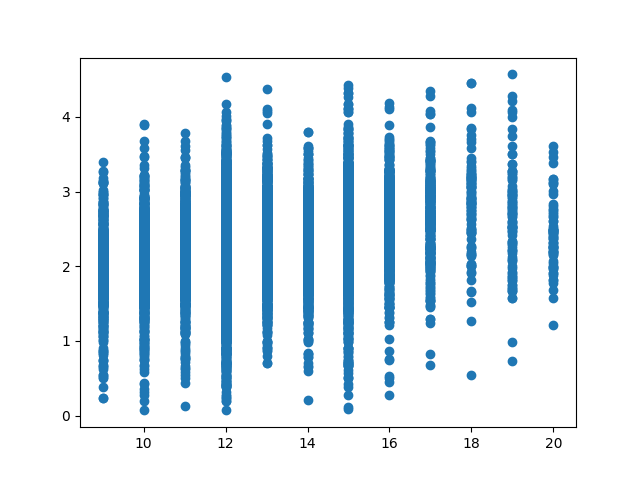
\includegraphics[width=0.8\textwidth]{assets/fig.png}
			      \caption{Histograma de la la gama simulada}
		      \end{figure}


		      \pagebreak

		      \begin{pythonbox}[Python Code]
			      \inputminted{python}{code/prob3b.py}
		      \end{pythonbox}


		\item One might suspect that the value of education is enhanced by greater ability. We could
		      examine this effect by introducing an interaction of the two variables in the equation.
		      Add the variable
		      $$
			      EducAb = Educ \times ability
		      $$
		      to the base model in part a. Now, what is the marginal value of an additional year of
		      education? The sample mean value of ability is 0.052374. Compute a confidence interval
		      for the marginal impact on ln Wage of an additional year of education for a person of
		      average ability.

		      \begin{table}[htbp]
			      \centering
			      \caption{OLS Regression Results: lwage}
			      \begin{tabular}{lcccccc}
				      \hline
				      \textbf{Variable}                    & \textbf{Coef.} & \textbf{Std. Err.}                               & \textbf{z} & \textbf{P$>|z|$} & \textbf{[0.025} & \textbf{0.975]} \\
				      \hline
				      Intercept                            & 1.0019         & 0.034                                            & 29.130     & 0.000            & 0.934           & 1.069           \\
				      edu                                  & 0.0701         & 0.002                                            & 28.353     & 0.000            & 0.065           & 0.075           \\
				      educab                               & 0.0025         & 0.002                                            & 1.202      & 0.229            & -0.002          & 0.007           \\
				      ability                              & 0.0469         & 0.026                                            & 1.824      & 0.068            & -0.003          & 0.097           \\
				      exper                                & 0.0395         & 0.001                                            & 43.684     & 0.000            & 0.038           & 0.041           \\
				      meduc                                & 5.423e-05      & 0.002                                            & 0.032      & 0.975            & -0.003          & 0.003           \\
				      feduc                                & 0.0053         & 0.001                                            & 3.949      & 0.000            & 0.003           & 0.008           \\
				      brokenhome                           & -0.0531        & 0.010                                            & -5.256     & 0.000            & -0.073          & -0.033          \\
				      siblings                             & 0.0048         & 0.002                                            & 2.689      & 0.007            & 0.001           & 0.008           \\
				      \hline
				      \multicolumn{7}{l}{\textit{Model statistics:}}                                                                                                                               \\
				      \multicolumn{2}{l}{R-squared}        & 0.176          & \multicolumn{4}{l}{}                                                                                                 \\
				      \multicolumn{2}{l}{Adj. R-squared}   & 0.176          & \multicolumn{4}{l}{}                                                                                                 \\
				      \multicolumn{2}{l}{F-statistic}      & 478.7          & \multicolumn{4}{l}{(Prob $F$-statistic = 0.000)}                                                                     \\
				      \multicolumn{2}{l}{No. Observations} & 17919          & \multicolumn{4}{l}{}                                                                                                 \\
				      \multicolumn{2}{l}{Df Residuals}     & 17910          & \multicolumn{4}{l}{}                                                                                                 \\
				      \multicolumn{2}{l}{Df Model}         & 8              & \multicolumn{4}{l}{}                                                                                                 \\
				      \multicolumn{2}{l}{Log-Likelihood}   & -12254         & \multicolumn{4}{l}{}                                                                                                 \\
				      \multicolumn{2}{l}{AIC}              & 2.453e+04      & \multicolumn{4}{l}{}                                                                                                 \\
				      \multicolumn{2}{l}{BIC}              & 2.460e+04      & \multicolumn{4}{l}{}                                                                                                 \\
				      \multicolumn{7}{l}{Durbin-Watson: 0.804}                                                                                                                                     \\
				      \multicolumn{7}{l}{Omnibus: 1115.367, Prob(Omnibus): 0.000}                                                                                                                  \\
				      \multicolumn{7}{l}{Jarque-Bera (JB): 2085.291, Prob(JB): 0.000}                                                                                                              \\
				      \multicolumn{7}{l}{Skew: -0.460, Kurtosis: 4.396}                                                                                                                            \\
				      \multicolumn{7}{l}{Cond. No.: 232}                                                                                                                                           \\
				      \hline
			      \end{tabular}
		      \end{table}

		      \begin{table}[htbp]
			      \centering
			      \caption{Predicted Change in Assaults}
			      \begin{tabular}{l c}
				      \hline
				      \textbf{Statistic}            & \textbf{Value} \\
				      \hline
				      Predicted change in assaults  & 0.07           \\
				      95\% Confidence Interval (CI) & [0.07, 0.08]   \\
				      \hline
			      \end{tabular}
		      \end{table}

		      \pagebreak

		      \begin{pythonbox}[Python Code]
			      \inputminted{python}{code/prob3c.py}
		      \end{pythonbox}
		\item Combine the models in (b) and (c). Add both $educ^2$ and $EducAb$ to the base model in
		      the beginning of the question and re-estimate. As before, report all results and describe
		      your findings. If we define low ability as less than the mean and high ability as greater
		      than the mean, the sample averages are $-0.798563$ for the 7,864 low-ability individuals in
		      the sample and $+0.717891$ for the 10,055 high-ability individuals in the sample. Using
		      the formulation in part (b), with this new functional form, sketch, describe, and compare
		      the log wage profiles for low- and high-ability individuals.

		      \begin{table}[htbp]
			      \centering
			      \caption{OLS Regression Results: lwage}
			      \begin{tabular}{lcccccc}
				      \hline
				      \textbf{Variable}                    & \textbf{Coef.} & \textbf{Std. Err.}                               & \textbf{z} & \textbf{P$>|z|$} & \textbf{[0.025} & \textbf{0.975]} \\
				      \hline
				      Intercept                            & -0.1051        & 0.154                                            & -0.683     & 0.494            & -0.407          & 0.196           \\
				      edu                                  & 0.2409         & 0.023                                            & 10.343     & 0.000            & 0.195           & 0.287           \\
				      edu2                                 & -0.0065        & 0.001                                            & -7.350     & 0.000            & -0.008          & -0.005          \\
				      educab                               & 0.0163         & 0.003                                            & 5.986      & 0.000            & 0.011           & 0.022           \\
				      ability                              & -0.1245        & 0.034                                            & -3.717     & 0.000            & -0.190          & -0.059          \\
				      exper                                & 0.0395         & 0.001                                            & 43.801     & 0.000            & 0.038           & 0.041           \\
				      meduc                                & 0.0005         & 0.002                                            & 0.264      & 0.792            & -0.003          & 0.004           \\
				      feduc                                & 0.0052         & 0.001                                            & 3.884      & 0.000            & 0.003           & 0.008           \\
				      brokenhome                           & -0.0478        & 0.010                                            & -4.710     & 0.000            & -0.068          & -0.028          \\
				      siblings                             & 0.0046         & 0.002                                            & 2.595      & 0.009            & 0.001           & 0.008           \\
				      \hline
				      \multicolumn{7}{l}{\textit{Model statistics:}}                                                                                                                               \\
				      \multicolumn{2}{l}{R-squared}        & 0.179          & \multicolumn{4}{l}{}                                                                                                 \\
				      \multicolumn{2}{l}{Adj. R-squared}   & 0.178          & \multicolumn{4}{l}{}                                                                                                 \\
				      \multicolumn{2}{l}{F-statistic}      & 439.1          & \multicolumn{4}{l}{(Prob $F$-statistic = 0.000)}                                                                     \\
				      \multicolumn{2}{l}{No. Observations} & 17919          & \multicolumn{4}{l}{}                                                                                                 \\
				      \multicolumn{2}{l}{Df Residuals}     & 17909          & \multicolumn{4}{l}{}                                                                                                 \\
				      \multicolumn{2}{l}{Df Model}         & 9              & \multicolumn{4}{l}{}                                                                                                 \\
				      \multicolumn{2}{l}{Log-Likelihood}   & -12225         & \multicolumn{4}{l}{}                                                                                                 \\
				      \multicolumn{2}{l}{AIC}              & 2.447e+04      & \multicolumn{4}{l}{}                                                                                                 \\
				      \multicolumn{2}{l}{BIC}              & 2.455e+04      & \multicolumn{4}{l}{}                                                                                                 \\
				      \multicolumn{7}{l}{Durbin-Watson: 0.806}                                                                                                                                     \\
				      \multicolumn{7}{l}{Omnibus: 1133.720, Prob(Omnibus): 0.000}                                                                                                                  \\
				      \multicolumn{7}{l}{Jarque-Bera (JB): 2158.151, Prob(JB): 0.000}                                                                                                              \\
				      \multicolumn{7}{l}{Skew: -0.460, Kurtosis: 4.429}                                                                                                                            \\
				      \multicolumn{7}{l}{Cond. No.: 7.41e+03}                                                                                                                                      \\
				      \hline
			      \end{tabular}
		      \end{table}

		      \begin{figure}[H]
			      \centering
			      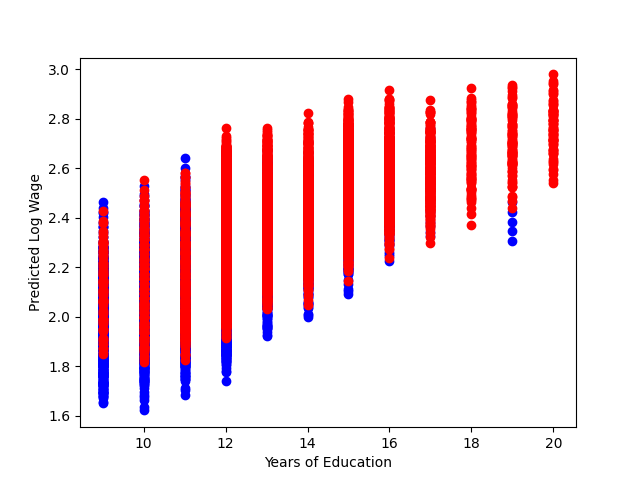
\includegraphics[width=0.8\textwidth]{assets/fig3.png}
			      \caption{Histograma de la la gama simulada}
		      \end{figure}



		      \begin{pythonbox}[Python Code]
			      \inputminted{python}{code/prob3d.py}
		      \end{pythonbox}


		\item Suppose that you are now given the following regression model:
		      \[
			      \begin{split}
				      \ln(\text{wage}) =   \beta_0 & + \beta_1  \text{educ} \times \mathbf{1}(\text{educ} < \tau) + \beta_2 \text{educ} \times \mathbf{1}(\text{educ} \ge \tau) + \beta_3 \text{exp} \\
				                                   & + \beta_4 \text{MotherEduc} + \beta_5 \text{FatherEduc} + \beta_6 \text{broken}                                                                 \\
				                                   & + \beta_7  \text{siblings} + \epsilon
			      \end{split}
		      \]
		      \noindent
		      where \( \tau \) is the threshold parameter, and
		      \[
			      \mathbf{1}(\text{Educ} < \tau) =
			      \begin{cases}
				      1 & \text{if } \text{Educ} < \tau, \\
				      0 & \text{otherwise}
			      \end{cases}
			      \quad \text{and} \quad
			      \mathbf{1}(\text{Educ} \ge \tau) =
			      \begin{cases}
				      1 & \text{if } \text{Educ} \ge \tau, \\
				      0 & \text{otherwise}.
			      \end{cases}
		      \]

		      \begin{table}[htbp]
			      \centering
			      \caption{OLS Regression Results: lwage}
			      \begin{tabular}{lcccccc}
				      \hline
				      \textbf{Variable}                    & \textbf{Coef.} & \textbf{Std. Err.}                               & \textbf{t} & \textbf{P$>|t|$} & \textbf{[0.025} & \textbf{0.975]} \\
				      \hline
				      Intercept                            & 0.9469         & 0.037                                            & 25.458     & 0.000            & 0.874           & 1.020           \\
				      tao1                                 & 0.0747         & 0.003                                            & 28.915     & 0.000            & 0.070           & 0.080           \\
				      tao2                                 & 0.0711         & 0.002                                            & 31.510     & 0.000            & 0.067           & 0.076           \\
				      ability                              & 0.0761         & 0.005                                            & 15.347     & 0.000            & 0.066           & 0.086           \\
				      exper                                & 0.0396         & 0.001                                            & 44.021     & 0.000            & 0.038           & 0.041           \\
				      meduc                                & 0.0002         & 0.002                                            & 0.091      & 0.928            & -0.003          & 0.003           \\
				      feduc                                & 0.0053         & 0.001                                            & 3.931      & 0.000            & 0.003           & 0.008           \\
				      brokenhome                           & -0.0519        & 0.010                                            & -5.192     & 0.000            & -0.071          & -0.032          \\
				      siblings                             & 0.0048         & 0.002                                            & 2.689      & 0.007            & 0.001           & 0.008           \\
				      \hline
				      \multicolumn{7}{l}{\textit{Model statistics:}}                                                                                                                               \\
				      \multicolumn{2}{l}{R-squared}        & 0.176          & \multicolumn{4}{l}{}                                                                                                 \\
				      \multicolumn{2}{l}{Adj. R-squared}   & 0.176          & \multicolumn{4}{l}{}                                                                                                 \\
				      \multicolumn{2}{l}{F-statistic}      & 479.4          & \multicolumn{4}{l}{(Prob $F$-statistic = 0.000)}                                                                     \\
				      \multicolumn{2}{l}{No. Observations} & 17919          & \multicolumn{4}{l}{}                                                                                                 \\
				      \multicolumn{2}{l}{Df Residuals}     & 17910          & \multicolumn{4}{l}{}                                                                                                 \\
				      \multicolumn{2}{l}{Df Model}         & 8              & \multicolumn{4}{l}{}                                                                                                 \\
				      \multicolumn{2}{l}{Log-Likelihood}   & -12251         & \multicolumn{4}{l}{}                                                                                                 \\
				      \multicolumn{2}{l}{AIC}              & 2.452e+04      & \multicolumn{4}{l}{}                                                                                                 \\
				      \multicolumn{2}{l}{BIC}              & 2.459e+04      & \multicolumn{4}{l}{}                                                                                                 \\
				      \multicolumn{7}{l}{Durbin-Watson: 0.804}                                                                                                                                     \\
				      \multicolumn{7}{l}{Omnibus: 1113.540, Prob(Omnibus): 0.000}                                                                                                                  \\
				      \multicolumn{7}{l}{Jarque-Bera (JB): 2094.899, Prob(JB): 0.000}                                                                                                              \\
				      \multicolumn{7}{l}{Skew: -0.457, Kurtosis: 4.404}                                                                                                                            \\
				      \multicolumn{7}{l}{Cond. No.: 235}                                                                                                                                           \\
				      \hline
			      \end{tabular}
		      \end{table}
		      \begin{pythonbox}[Python Code]
			      \inputminted{python}{code/prob3e.py}
		      \end{pythonbox}
	\end{enumerate}
\end{homeworkProblem}

\begin{homeworkProblem}
	Using the \textbf{California test score date}, estimate the regression below using
	Nonlinear Least Squares. Report you coefficient estimates and standard errors.
	$$
		TestScore = \beta_0 (1- e^{\beta_1(income - \beta_2)}) + \epsilon
	$$
\end{homeworkProblem}


\begin{homeworkProblem}
	Use the \textbf{Consumption.xlsx}. We have previously estimated the nonlinear consuption
	function below using nonlinear least squares in class:
	$$
		C = \alpha + \beta Y^{\gamma} + \epsilon
	$$
	Where $C$ is the real consumption and $Y$ is the real disposable income. Alternatively, we can
	assume that the error term has a normal distribution and estimate the nonlinear regression
	above using the maximum likeligood estimation (MLE) approach, In particular, the MLE
	approach maximizes the log-likelihood function given by:
	$$
		L(\alpha, \beta, \gamma, \sigma^2) = -\frac{n}{2} \log(\sigma^2) - \log(2\pi) - \frac{1}{2 \sigma^2} \sum_{i=1}^{n}(C_i - \alpha - \beta Y^{\gamma})^2
	$$
	Where $\sigma^2$ is the variance of the error term. Using a statistical programming language of you choice,
	estimate the regression model using the maximum likelihood estimation approach. Your estimate are expected to
	be similar to those in Table 7.1 of Green's textbook. Please submit the following:
	\begin{enumerate}[(a)]
		\item Your code used to preform the estimation.
		\item The output of your estimation, including the estimated parameters and the error variance.
	\end{enumerate}
\end{homeworkProblem}

\end{document}
